\documentclass{article}
\usepackage[utf8]{inputenc}
\setlength{\parindent}{0em}
\setlength{\parskip}{1.4ex}
\usepackage[danish]{babel}
\usepackage[utf8]{inputenc}
\usepackage{graphicx}
\graphicspath{{pictures/}}
\usepackage{mathtools}
\usepackage{amsfonts,amsmath,amssymb,amsthm} 
\newtheorem{theorem}{Sætning}

\title{DM500 Eksamensopgave}

\author{
	Thomas Urup Schjerlund\\
	\texttt{thsch20@student.sdu.dk}
	\and
	Tobias Klink Lehn\\
	\texttt{toleh20@student.sdu.dk}
	\and
	Philip Hayberg Thomsen\\
	\texttt{phtho20@student.sdu.dk}
	\and
	Sean Chrone Græns\\
	\texttt{segra20@student.sdu.dk}
}
\date{15. November 2020}

\begin{document}

\begin{titlepage}
\maketitle
\end{titlepage}

\section{Reeksamen DM527 Opg 1 - Tobias}
\begin{figure}[h]
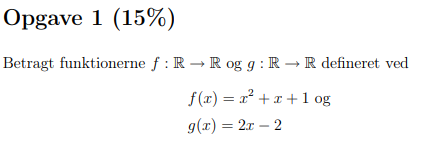
\includegraphics[scale=1]{Opgave1Formulering}
\end{figure}

\begin{figure}[h]
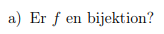
\includegraphics[scale=1]{opga}
\end{figure}
\textbf{Svar:}
En afbildning, $\phi: A \rightarrow B$ er bijektiv, hvis og kun hvis funktionen både er \emph{injektiv} (one-to-one) og \emph{surjektiv} (onto).

\begin{theorem}
$f$ er injektiv, hvis $\forall x_1, x_2 \in Dm(f): x_1 \neq x_2 \rightarrow f(x_1) \neq f(x_2)$
\end{theorem}

Sagt på en anden måde, så skal det for alle værdier af x i definitionsmængden gælde, at x hvis to x-værdier er forskellige fra hinanden, så er deres funktionsværdier det også. Helt basalt vil det sige, at to x-værdier ikke kan dele en y-værdi.

Ved at indsætte $x_1$ og $x_2$ og sætte deres funktionsværdi lig hinanden, kan det afgøres hvorvidt det også betyder, at x-værdierne var ens til at starte med - det skal de være, hvis funktionen skal være injektiv:
\begin{center}
\[f(x_1) = x_1^2 + x_1 + 1 \] 
\[ f(x_2)=x_2^2 + x_2 + 1 \] 
\begin{align*}
f(x_1) = f(x_2) \\
\Rightarrow x^2_1 + x_1 + 1 = x^2_2 + x_2 + 1 && \text{Funktionsværdien indsættes} \\
\Leftrightarrow x^2_1 + x_1 = x^2_2 + x_2 && \text{1 går ud på begge sider} \\
\Leftrightarrow x_1^2 = x_2^2 + x_2 - x_1 && \text{$x_1$ trækkes fra på begge sider}\\
\Rightarrow x_1 = \pm\sqrt{x_2^2 + x_2 - x_1} \\
\Rightarrow x_1 = \pm\sqrt{k}  && \text{, $k \in \mathbb{R}$}
\end{align*}
\end{center}

Da det hurtigt viser sig at $x_1 \neq k \Rightarrow f(x_1) = f(k)$, må det betyde, at $x_1$ kan have samme funktionsværdi som et andet tal (forskelligt fra $x_1$) i definitonsmængden ($Dm(f) = \mathbb{R}$), og derfor er \emph{f} ikke injektiv, og derfor automatisk heller ikke bijektiv. For at understrege pointen kan man forsøge sig med $x_1 = 4.91$ og $x_2 = -5.91$ og derfor få:

\begin{align*}
\begin{split}
f(4) = 4.91^2 + 4.91 + 1 \approx 30.02  \\
f(-5.91) = (-5.91)^2 + 5.91 + 1 \approx 30.02
\end{split}
\end{align*}
Af den grund behøver vi ikke kontrollere, om \emph{f} er surjektiv.


\begin{figure}[h]
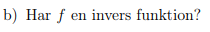
\includegraphics[scale=1]{opgb}
\end{figure}

En funktion \emph{f} har en invers, hvis og kun hvis f er bijektiv. Da vi tidligere har konkluderet at \emph{f} ikke er bijektiv, må det også være tilfældet, at \emph{f} ikke er invertibel og derfor ikke har nogen invers.

\begin{figure}[h]
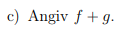
\includegraphics[scale=1]{opgc}
\end{figure}
To funktioner kan adderes ved at addere deres funktionsforskrifter ved brug af standard algebraiske regler
\begin{align*}
(f+g)(x) = f(x) + g(x) \\
\Rightarrow (f+g)(x) = (x^2 + x + 1) + (2x - 2) && \text{f og g indsættes på deres pladser} \\
= x^2 + x + 1 + 2x - 2 && \text{Parentser fjernes, da der kun indgår + mellem dem} \\
= x^2 + 3x - 1 \\
\end{align*}

\begin{figure}[h]
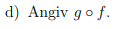
\includegraphics[scale=1]{opgd}
\end{figure}
Den sammensatte funktion $f \circ g$ beregnes på følgende vis:
\par
\begin{center}
\begin{math}
f \circ g = f(g(x))
\end{math}
\end{center}

Indsætter man $f$ i $g$ fås:
\begin{center}
\begin{align*}
g(f(x)) = g(x^2 + x + 1) \\
= 2 \cdot (x^2 + x + 1) - 2 && \text{udtrykket indsættes i g} \\
= 2x^2 + 2x + 2 - 2 && \text{Parentesen udregnes} \\
= 2x^2 + 2x
\end{align*}
\end{center}

Dette var løsningen til Opgave 1 i DM527 Reeksamen, Januar 2012.

\section{- Thomas}

\section{- Phillip}

\section{Reeksamen DM549 Februar 2015 Opg 3 - Sean }
\subsection{Opgave 3}
Lad R, S og T være binære relationer på mængden {1, 2, 3, 4}.


\subsubsection{Opgave A}
Lad \[R = \{(1, 1),(2, 1),(2, 2),(2, 4),(3, 1),(3, 3),(3, 4),(4, 1),(4, 4)\}\]

Er R en partiel ordning?

\textbf{Svar:}
{En partiel ordning er en \emph{relation}, $R$, på en mængde,  hvor $R$ er refleksiv, anti-symmetrisk og transitiv. Det bedømmes hvorvidt $R$ besidder disse egenskaber:}


\subsubsubsection{Refleksivitet:}
Da sætningen \[\forall a \in A : (a,a) \in R\] betyder at en refleksiv ordning skal relatere enhver værdi til sig selv og da denne er opfyldt kan første krav til en partiel ordning krydses af.





\subsubsubsection{Antisymmetri:}
Hvis en ordning skal være antisymmetrisk gælder at \[\forall a, b \in A \land a \neq b: aRb \Rightarrow a\cancel{R}b\]\\

Her forstås at  Hvis a er relateret til b kan b ikke være relateret til a, medmindre a = b
En anden måde at se om en mængde er antisymmetrisk er ved hjælp af en matrice.\\
\textbf{Matrice for R:}\\ 


\[R=\begin{bmatrix}
1 & 0 & 0 & 0\\
1 & 1 & 0 & 0\\
1 & 0 & 1 & 1\\
1 & 0 & 0 & 1
\end{bmatrix}\]


Sammenligner man værdierne diagonalt og man har en forskellig værdi. Gælder dog ikke to ens 0-værdier, da de i så fald ikke er relateret til hinanden på nogen vis, er relationen antisymmetrisk. 

Her kan man se at R altså er antisymmetrisk.

\subsubsubsection{Transitivitet:}
Her gælder at \[(a,b)\in R \wedge (b,c)\in R \Rightarrow (a,c)\in R, \;  \forall a,b,c \in A\]
Her har vi en binær relation med mængden 1, 2, 3, 4 hvilken betyder at hvis relationen skal være transitiv, skal alle mægnde værdier være i relation med hinanden.
Den transitive lukning ser således ud for relationen \[t(R) = \{(1,1), (2,1), (2,2), (2,4), (3,1), (3,3), (3,4), (4,1), (4,4)\} \cup \{(2,3)\}\]
Her kan vi se relationen forenet med en ny relation, nemlig (2,3), er den transitive lukning af $R$. Af den grund var $R$ ikke transitiv til at starte med, da elementet (2,3) manglede. Da denne ikke er en del a relationen R kan den ikke kaldes transitiv, og dermed er den ikke en partiel ordning.

\vspace{2cm}


\subsubsection{Opgave B}
Lad \[S = \{(1, 2),(2, 3),(2, 4),(4, 2)\}\]


Angiv den transitive lukning af S?
\\\textbf{Svar:}


Som tidligere forklaret er den transitive lukning, samlingen af relationer som der kræves for at relatere enhver værdi med enhver anden. Altså \[(a,b)\in R \wedge (b,c)\in R \Rightarrow (a,c)\in R, \;  \forall a,b,c \in A\]

Altså er lukningen også beksrevet som \[S^*=\bigcup_{i=1}^{\infty} S^i\]

Er der en vej fra den oprindelige relation, kommer der en direkte vej i lukningen.

Har $T$ $n$ elementer kan man skrive \[S^*=\bigcup_{i=1}^{|A|} S^4 = t(S)= \{(1, 2),(2, 3),(2, 4),(4, 2)\}. \cup \{(1,3), (1,4),\} \cup \{(3,4)\}\]



\textbf{Matrice for S:}\\

\[S=\begin{bmatrix}
0 & 1 & 0 & 0\\
0 & 0 & 1 & 1\\
0 & 0 & 0 & 0\\
0 & 1 & 0 & 0
\end{bmatrix}\\\]



\subsubsection{Opgave C}

Lad \[T = {(1, 1),(1, 3),(2, 2),(2, 4),(3, 1),(3, 3),(4, 2),(4, 4)}\]

Bemærk, at T er en ækvivalens-relation.
Angiv T's ækvivalens-klasser.

Ækvivalens relationer er relationer der er både symmetriske, transitive og refleksive. 

\textbf{Ækvivalens-klasserne for T som følger \[[a] = \{b \vert (a,b) \in R\}\\\]}



\[[1]=\{1,3\}\]
\[[2]=\{2,4\}\\\]

og da \[[1]=[3], [2]=[4]\] fordi \[a\subseteq b\] \[c \in [a] \Rightarrow aRc \Rightarrow bRc \Rightarrow c\in [b]\]
indgår disse i samme klasse.\\

\textbf{Matrice T:}\\

\[T=\begin{bmatrix}
1 & 0 & 1 & 0\\
0 & 1 & 0 & 1\\
1 & 0 & 1 & 0\\
0 & 1 & 1 & 0
\end{bmatrix}\\\]


\end{document}
